\documentclass{article} % For LaTeX2e
\usepackage{nips14submit_e,times}
\usepackage{amsmath}
\usepackage{amsthm}
\usepackage{amssymb}
\usepackage{mathtools}
\usepackage{hyperref}
\usepackage{url}
\usepackage{algorithm}
\usepackage[noend]{algpseudocode}
%\documentstyle[nips14submit_09,times,art10]{article} % For LaTeX 2.09

\usepackage{bbm}
\usepackage{graphicx}
\usepackage{caption}
\usepackage{subcaption}
\usepackage{MnSymbol}

\def\eQb#1\eQe{\begin{eqnarray*}#1\end{eqnarray*}}
\def\eQnb#1\eQne{\begin{eqnarray}#1\end{eqnarray}}
\providecommand{\e}[1]{\ensuremath{\times 10^{#1}}}
\providecommand{\pb}[0]{\pagebreak}
\DeclarePairedDelimiter\ceil{\lceil}{\rceil}
\DeclarePairedDelimiter\floor{\lfloor}{\rfloor}

\newcommand{\E}{\mathrm{E}}
\newcommand{\Var}{\mathrm{Var}}
\newcommand{\Cov}{\mathrm{Cov}}
\newcommand\eqD{\stackrel{\mathclap{\normalfont\mbox{d}}}{=}}

\def\Qb#1\Qe{\begin{question}#1\end{question}}
\def\Sb#1\Se{\begin{solution}#1\end{solution}}

\newenvironment{claim}[1]{\par\noindent\underline{Claim:}\space#1}{}
\newtheoremstyle{quest}{\topsep}{\topsep}{}{}{\bfseries}{}{ }{\thmname{#1}\thmnote{ #3}.}
\theoremstyle{quest}
\newtheorem*{definition}{Definition}
\newtheorem*{theorem}{Theorem}
\newtheorem*{lemma}{Lemma}
\newtheorem*{question}{Question}
\newtheorem*{preposition}{Preposition}
\newtheorem*{exercise}{Exercise}
\newtheorem*{challengeproblem}{Challenge Problem}
\newtheorem*{solution}{Solution}
\newtheorem*{remark}{Remark}
\usepackage{verbatimbox}
\usepackage{listings}
\usepackage{mathrsfs}
\title{ProbLimI: \\
Problem Set VI}


\author{
Youngduck Choi \\
CIMS \\
New York University\\
\texttt{yc1104@nyu.edu} \\
}


% The \author macro works with any number of authors. There are two commands
% used to separate the names and addresses of multiple authors: \And and \AND.
%
% Using \And between authors leaves it to \LaTeX{} to determine where to break
% the lines. Using \AND forces a linebreak at that point. So, if \LaTeX{}
% puts 3 of 4 authors names on the first line, and the last on the second
% line, try using \AND instead of \And before the third author name.

\newcommand{\fix}{\marginpar{FIX}}
\newcommand{\new}{\marginpar{NEW}}

\nipsfinalcopy % Uncomment for camera-ready version

\begin{document}


\maketitle

\begin{abstract}
This work contains solutions to the exercises of the problem set V. The
chosen problems are 1,2, and 3.
\end{abstract}

\bigskip

\begin{question}[1]
\hfill
\begin{figure}[h!]
  \centering
    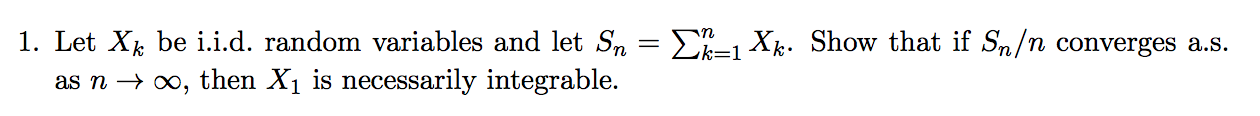
\includegraphics[width=0.7\textwidth]{prob-e8-p1.png}
\end{figure}
\end{question}
\begin{solution} \hfill \\
We first prove the following lemma: if $Y \geq 0$ and $p > 0$, then
$\mathbb{E}(Y^p) = \int_{0}^{\infty} py^{p-1}P(Y > y) dy$. 

\smallskip

By Tonelli,
\eQb
\int_{0}^{\infty} py^{p-1}\mathbb{P}(Y > y) dy &=& \int_{0}^{\infty} \int_{\Omega}
py^{p-1}1_{\{Y > y \} } dP dy = 
\eQe

We first prove the following lemma: if $\{X_n\}$ are i.i.d. with $\mathbb{E}|X_1| = 
\infty$, then $\mathbb{P}(\dfrac{S_n}{n} \>\>\> \text{converges}) = 0$. 
From 2.2.
\eQb
\mathbb{E}|X_1| = \int_{0}^{\infty} \mathbb{P}(|X_1| > x) dx &\leq& 
\sum_{n=0}^{\infty} \mathbb{P}(|X_1| > n).
\eQe
As $\mathbb{E}|X_1| = \infty$, $\sum_{n=0}^{\infty} \mathbb{P}(|X_1| > n) = \infty$,
and by Borel Cantelli II, 
\eQb
\mathbb{P}(|X_n| \geq n \>\> \text{i.o.}) &=& 1. 
\eQe
Now, it suffices to show that 
\eQb
\{ \dfrac{S_n}{n} \>\>\> \text{converges}\} &\subset& 
\{ |X_n \geq n \>\> \text{i.o.}\}.
\eQe

Suppose for sake of contradiction that $\mathbb{E}|X_1|= \infty$. Then, by
the lemma,  
\eQb
\mathbb{P}(\dfrac{S_n}{n} \>\>\> \text{converges}) &=& 0 
\eQe
which is a contradiction. Hence, $\mathbb{E}|X_1| < \infty$, i.e. $X_1$ is integrable.
 
\end{solution}

\begin{question}[2]
\hfill
\begin{figure}[h!]
  \centering
    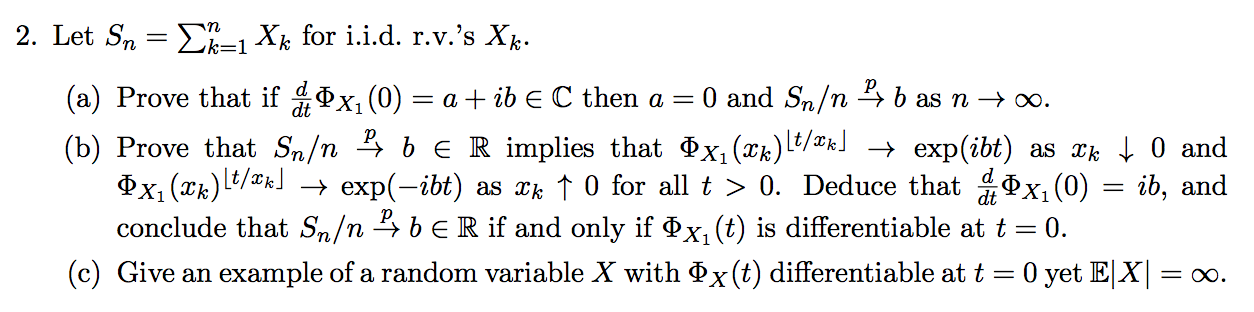
\includegraphics[width=0.7\textwidth]{prob-e8-p2.png}
\end{figure}
\end{question}
\begin{solution} \hfill \\
\end{solution}

\newpage

\begin{question}[2]
\hfill
\begin{figure}[h!]
  \centering
    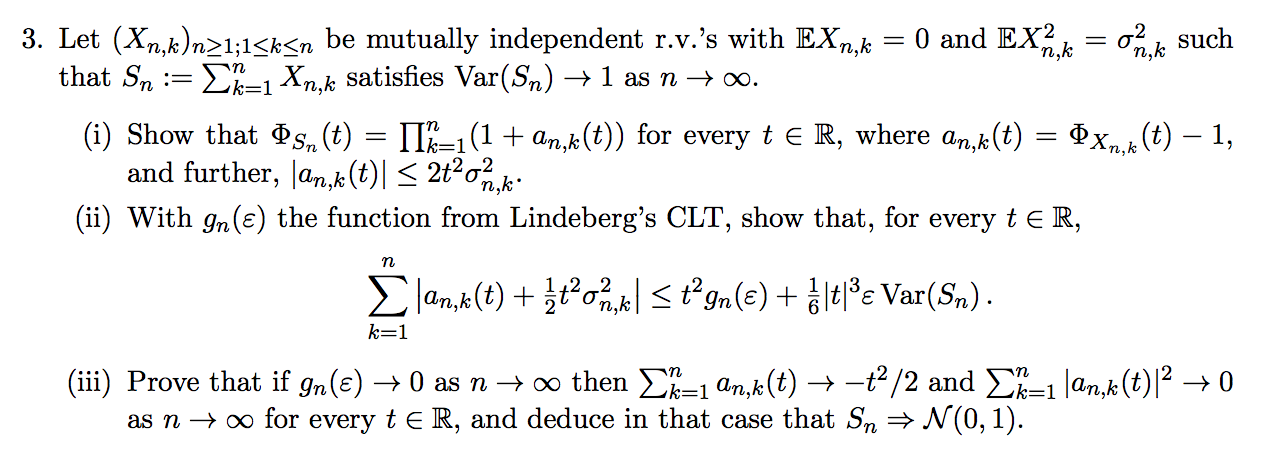
\includegraphics[width=0.7\textwidth]{prob-e8-p3.png}
\end{figure}
\end{question}
\begin{solution} \hfill \\
\end{solution}

\newpage

\begin{question}[4]
\hfill
\begin{figure}[h!]
  \centering
    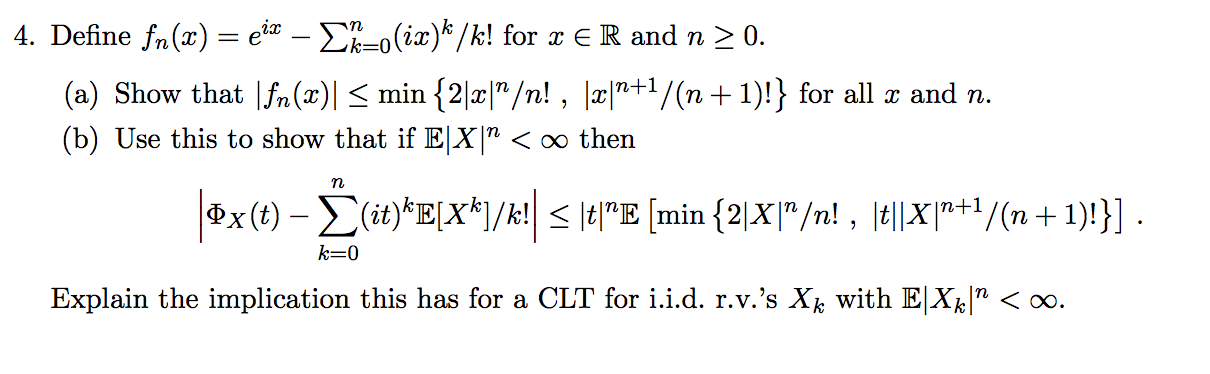
\includegraphics[width=0.7\textwidth]{prob-e8-p4.png}
\end{figure}
\end{question}
\begin{solution} \hfill \\
Let $x \in \mathbb{R}$. By integration by parts,
\eQnb 
\int_{0}^{x} (x-s)^n e^{is} ds &=& \dfrac{x^{n+1}}{n+1} + \dfrac{i}{n+1}
\int_{0}^{x} (x-s)^{n+1}e^{is} ds
\eQne \label{eq:4}

for each $n \geq 0$. If $n = 0$, then
\eQb
x + i \int_{0}^{x} (x-s)e^{is} ds &=& \int_{0}^{x} e^{is}ds = \dfrac{e^{ix} - 1}{i} 
\eQe
and hence
\eQb
e^{ix} = 1 + ix + i^{2} \int_{0}^{x} (x-s)e^{is} ds. 
\eQe
Suppose for some $n > 0$
\eQnb
e^{ix} - \sum_{k=0}^{n} \dfrac{(ix)^k}{k!} &=& \dfrac{i^{n+1}}{n!} \int_{0}^{x}
(x-s)^n e^{is} ds  
\eQne \label{eq:4.1}

Then, combined with \eqref{eq:4},
\eQb
e^{ix} - \sum_{k=0}^{n+1} \dfrac{(ix)^{k}}{k!} 
&=& \dfrac{i^{n+1}}{n!} \int_{0}^{x} (x-s)^n e^{is} ds - \dfrac{(ix)^{n+1}}{(n+1)!} \\
&=& \dfrac{i^{n+1}}{n!}(\int_{0}^{x} (x-s)^n e^{is} ds - \dfrac{x^{n+1}}{(n+1)} \\
&=& \dfrac{i^{n+2}}{(n+1)!} \int_{0}^{x} (x-s)^{n+1} e^{is} ds. 
\eQe
Hence, by induction, \eqref{eq:4.1} holds for all $n \geq 0$. If  $x \geq 0$, then
\eQb
|\dfrac{i^{n+1}}{n!} \int_{0}^{x} (x-s)^n e^{is} ds| &\leq&
\dfrac{1}{n!} \int_{0}^{x} |(x-s)^n| ds = \dfrac{1}{n!} \int_{0}^{x} 
(x-s)^n ds = \dfrac{1}{(n+1)!} |x|^{n+1}.
\eQe
If $x < 0$, then
\eQb
|\dfrac{i^{n+1}}{n!} \int_{0}^{x} (x-s)^n e^{is} ds| &=&
|\dfrac{i^{n+1}}{n!} \int_{x}^{0} (x-s)^n e^{is} ds|
\leq
\dfrac{1}{n!} \int_{x}^{0} |(x-s)^n e^{is}| ds \\
&\leq&
\dfrac{1}{n!} \int_{x}^{0} (s-x)^n  ds = \dfrac{1}{(n+1)!} (-x)^{n+1} 
= \dfrac{1}{(n+1)!}|x|^{n+1}.
\eQe
Therefore,
\eQb
|f_n(x)| &\leq& \dfrac{1}{(n+1)!} |x|^{n+1} 
\eQe
for any $n \geq 0$. Now, again by integration by parts,
\eQb
\dfrac{i}{n} \int_{0}^{x} (x-s)^{n} e^{is} ds &=& -\dfrac{x^n}{n} + \int_{0}^{x}
(x-s)^{n-1} e^{is} ds 
\eQe
and hence
\eQb
\dfrac{i^{n+1}}{n!} \int_{0}^{x} (x-s)^{n} e^{is} ds = \dfrac{i^n}{(n-1)!}
\int_{0}^{x} (x-s)^{n-1}(e^{is} - 1) ds
\eQe
for any $n \geq 1$. If $x \geq 0$, then
\eQb
|\dfrac{i^{n+1}}{n!} \int_{0}^{x} (x-s)^{n} e^{is} ds| &=& |\dfrac{i^n}{(n-1)!} 
\int_{0}^{x} (x-s)^{n-1} (e^{is}  - 1) ds| \\
&\leq& \dfrac{1}{(n-1)!} \int_{0}^{x} |(x-s)^{n-1}||e^{is} - 1| ds \\
&\leq& \dfrac{2}{(n-1)!} \int_{0}^{x} (x-s)^{n-1} ds = \dfrac{2}{n!} |x|^{n}. 
\eQe
If $ x < 0$, then
\eQb
|\dfrac{i^{n+1}}{n!} \int_{0}^{x} (x-s)^{n} e^{is} ds| &=& |\dfrac{i^n}{(n-1)!} 
\int_{0}^{x} (x-s)^{n-1} (e^{is}  - 1) ds| \\
&\leq& \dfrac{1}{(n-1)!} \int_{0}^{x} |(x-s)^{n-1}||e^{is} - 1| ds \\
&\leq& \dfrac{2}{(n-1)!} \int_{0}^{x} (x-s)^{n-1} ds = \dfrac{2}{n!} |x|^{n}. 
\eQe
\end{solution}


\end{document}
